%%
%% This is file `sample-authordraft.tex',
%% generated with the docstrip utility.
%%
%% The original source files were:
%%
%% samples.dtx  (with options: `authordraft')
%% 
%% IMPORTANT NOTICE:
%% 
%% For the copyright see the source file.

%% 
%% Any modified versions of this file must be renamed
%% with new filenames distinct from sample-authordraft.tex.
%% 
%% For distribution of the original source see the terms
%% for copying and modification in the file samples.dtx.
%% 
%% This generated file may be distributed as long as the
%% original source files, as listed above, are part of the
%% same distribution. (The sources need not necessarily be
%% in the same archive or directory.)
%%
%% The first command in your LaTeX source must be the \documentclass command.
\documentclass[sigconf, review, anonymous]{acmart}

\makeatletter
\DeclareFontEncoding{LS1}{}{}
\makeatletter
\DeclareFontSubstitution{LS1}{stix}{m}{n}

\DeclareSymbolFont{symbols2}      {LS1}{stixfrak} {m} {n}

\DeclareMathSymbol{\leftouterjoin}            {\mathop}   {symbols2}{"11}
\DeclareMathSymbol{\rightouterjoin}           {\mathop}   {symbols2}{"12}
\DeclareMathSymbol{\fullouterjoin}            {\mathop}   {symbols2}{"13}
\DeclareMathSymbol{\innerjoin}                     {\mathop}   {symbols2}{"ED}

\newcommand{\sparql}{\textbf{SPARQL }}

%%
%% \BibTeX command to typeset BibTeX logo in the docs
\AtBeginDocument{%
  \providecommand\BibTeX{{%
    \normalfont B\kern-0.5em{\scshape i\kern-0.25em b}\kern-0.8em\TeX}}}

%% Rights management information.  This information is sent to you
%% when you complete the rights form.  These commands have SAMPLE
%% values in them; it is your responsibility as an author to replace
%% the commands and values with those provided to you when you
%% complete the rights form.
\setcopyright{acmcopyright}
\copyrightyear{2020}
\acmYear{2020}
\acmDOI{10.1145/1122445.1122456}

%% These commands are for a PROCEEDINGS abstract or paper.
\acmConference[Woodstock '18]{Woodstock '18: ACM Symposium on Neural
  Gaze Detection}{June 03--05, 2018}{Woodstock, NY}
\acmBooktitle{Woodstock '18: ACM Symposium on Neural Gaze Detection,
  June 03--05, 2018, Woodstock, NY}
\acmPrice{15.00}
\acmISBN{978-1-4503-9999-9/18/06}


%%
%% Submission ID.
%% Use this when submitting an article to a sponsored event. You'll
%% receive a unique submission ID from the organizers
%% of the event, and this ID should be used as the parameter to this command.
%%\acmSubmissionID{123-A56-BU3}

%%
%% The majority of ACM publications use numbered citations and
%% references.  The command \citestyle{authoryear} switches to the
%% "author year" style.
%%
%% If you are preparing content for an event
%% sponsored by ACM SIGGRAPH, you must use the "author year" style of
%% citations and references.
%% Uncommenting
%% the next command will enable that style.
%%\citestyle{acmauthoryear}

%%
%% end of the preamble, start of the body of the document source.
\begin{document}

%%
%% The "title" command has an optional parameter,
%% allowing the author to define a "short title" to be used in page headers.
\title{RDFFrames: Tidying knowledge graphs for Data Science Applications}

%%
%% The "author" command and its associated commands are used to define
%% the authors and their affiliations.
%% Of note is the shared affiliation of the first two authors, and the
%% "authornote" and "authornotemark" commands
%% used to denote shared contribution to the research.
\author{Aisha Mohamed}
%\authornote{Both authors contributed equally to this research.}
\email{}
\orcid{}
\author{}
%\authornotemark[1]
\affiliation{%
  \institution{}
  \streetaddress{}
  \city{}
  \state{}
  \postcode{}
}

\author{Ghadeer}
%\authornote{Both authors contributed equally to this research.}
\email{}
\orcid{}
\author{}
%\authornotemark[1]
\affiliation{%
  \institution{}
  \streetaddress{}
  \city{}
  \state{}
  \postcode{}
}

\author{Zoi}
%\authornote{Both authors contributed equally to this research.}
\email{}
\orcid{}
\author{}
%\authornotemark[1]
\affiliation{%
  \institution{}
  \streetaddress{}
  \city{}
  \state{}
  \postcode{}
}

\author{Abdu}
%\authornote{Both authors contributed equally to this research.}
\email{}
\orcid{}
\author{}
%\authornotemark[1]
\affiliation{%
  \institution{}
  \streetaddress{}
  \city{}
  \state{}
  \postcode{}
}


%%
%% By default, the full list of authors will be used in the page
%% headers. Often, this list is too long, and will overlap
%% other information printed in the page headers. This command allows
%% the author to define a more concise list
%% of authors' names for this purpose.
\renewcommand{\shortauthors}{}

%%
%% The abstract is a short summary of the work to be presented in the
%% article.
\begin{abstract}
\end{abstract}

%%
%% The code below is generated by the tool at http://dl.acm.org/ccs.cfm.
%% Please copy and paste the code instead of the example below.
%%

%%
%% Keywords. The author(s) should pick words that accurately describe
%% the work being presented. Separate the keywords with commas.
\keywords{}

%% A "teaser" image appears between the author and affiliation
%% information and the body of the document, and typically spans the
%% page.
%\begin{teaserfigure}
%  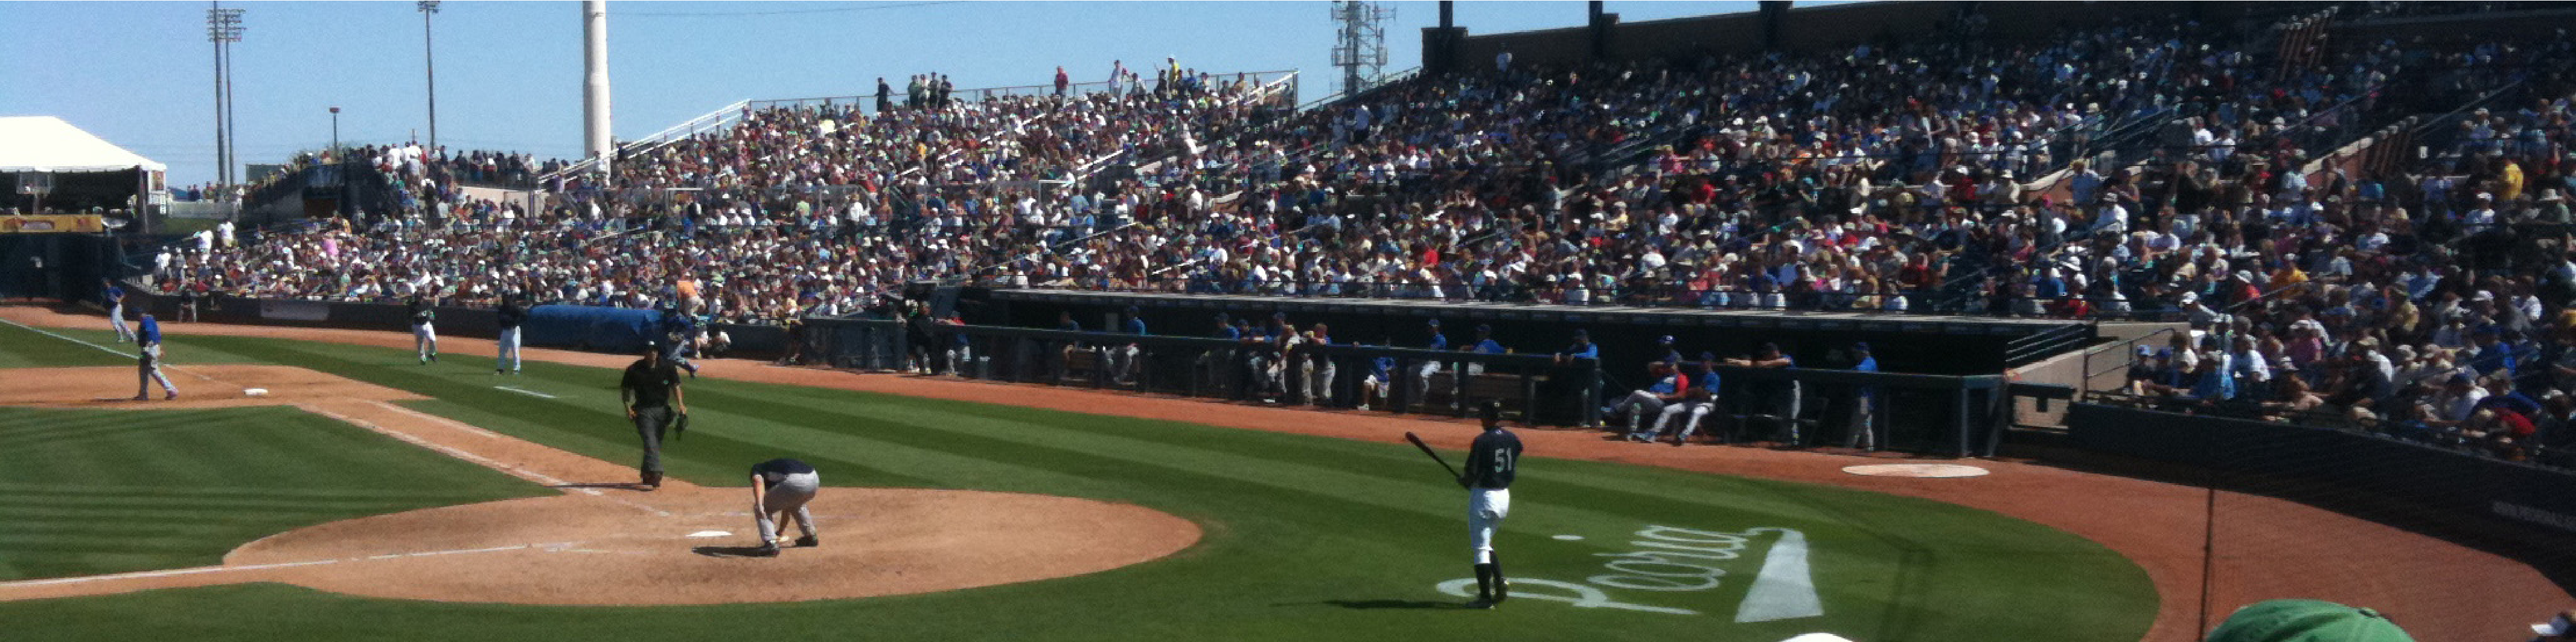
\includegraphics[width=\textwidth]{samples/sampleteaser}
%  \caption{Seattle Mariners at Spring Training, 2010.}
%  \Description{Enjoying the baseball game from the third-base
%  seats. Ichiro Suzuki preparing to bat.}
%  \label{fig:teaser}
%\end{teaserfigure}

%%
%% This command processes the author and affiliation and title
%% information and builds the first part of the formatted document.
\maketitle

\section{Introduction}
%!TEX root = main.tex

% Paragraph1: introducing the RDF data and the need to analyze them. Main ideas:
%1- many graph datasets are encoded in the RDF model 2- it has been integrated in many artificial intelligence applications (both traditional machine learning and relational learning models) so we need to facilitate data science and machine learning on top of them.
There has been a sharp growth in the number of graph datasets that are made available using the RDF\footnote{\url{https://www.w3.org/RDF}} (Resource Description Framework) data model.
Examples include knowledge graphs that cover a broad set of domains such as DBpedia~\cite{lehmann2015dbpedia}, YAGO~\cite{yago2}, and Wikidata~\cite{vrandecic12wikidata}, as well as specialized graphs for specific domains like social media networks, protein interaction networks, and bibliographic datasets. These datasets have been deployed in artificial intelligence applications including recommendation systems, search systems, virtual assistants and question answering. 

% Paragraph 2: to make it accessible for machine learning and data analysis, a lot of data querying and cleaning has to be done to convert it to the tidy data format. the tidy data format makes in an easy and efficient way to process data starting form a standard especially that RDF data is more heterogeneous, incomplete and noisy compared to relational tables
The RDF model provided a powerful abstraction for representing heterogeneous, noisy and incomplete data  which are characteristics of most real world datasets especially knowledge graphs that are automatically extracted from unreliable sources. However, it has complicated the already challenging and time consuming task of cleaning and preparing the data for analysis. It has been reported that $80\%$ of data analysis time and effort is spent on the process of exploring, cleaning and preparing the data.  \cite{dasu2003exploratory}. % I want to add a figure to represent the steps for analyzing the datasets in general. 1- data collection which is done in already in some specialized datasets and our API can be used to do it by navigating knowledge graphs. 
%2- exploring the data (exploratory analysis) and feature selection: finding the number of unique values for each attribute, finding the distribution of the values, finding the correlation between one attribute and the predicted feature or clustering. This helps us in finding the most wieldy target parameter to predict and the features that are fruteful and then querying it to extract the relevant information
%3- structuring it in tidy data format so that data cleaning can be done using data science frameworks
% 4- data cleaning
% 5- prepossessing: splitting into train valid and test, tokenization (converting things to integers), making sure input is of the same length, removing duplicates  
% 5- Analysis, visualization, Model Development and Evaluation
The difficulty can be attributed to the diverse and wide tasks that need to be done as depicted in Figure 1 which represents a typical data science task. The data scientist first has to collect the data from multiple resources to build a dataset, then do some exploratory analysis to find the main types of instances, their attributes, analyze data distribution, define the most feasible prediction tasks and identify the fruitful features to consider. Guided by the exploratory analysis, the scientist needs to query the dataset to extract the relevant information and structure it in the standard tidy data (Dataframe) format so that cleaning and pre-processing tasks can be carried out by data science frameworks easily and efficiently \cite{tidydata}. The Dataframe abstraction bridges the gap between the data extraction and the data analysis tools and can be easily integrated with most of the state of the art analysis and machine learning tools that consume the input data as a Dataframe. The tidy data philosophy has been realized by the DataFrame data structure where each table represents one type of instances and each column represents an attribute of that type of instances and each row is values of the attributes for one instance.

% Paragraph 3: What is available now? now accessing it is done in \sparql which is hard to learn, has ambiguous semantics and still needs to be imported to analysis tools. 
Currenlty, there are two main RDF data extraction tools. First, the data is queried using \sparql, the standard query language for RDF data, by either loading the data into a local RDF engine and
querying it~\cite{rdf-3x} or by issuing the query  
to a public SPARQL endpoint hosting the data. The sparql query solution is then exported to one of the familiar tabular formats using scripts that deal with the scalability and communication issues manually. 
The second is writing ad-hoc scripts to process the graph and extract the required tabular information from it and importing it to the tidy data format. The first solution requires the user to learn a new query language, which involves a steep and time-consuming learning curve and requires manually importing the output of the data extraction tool \sparql to the data cleaning, processing, analysis and visualization tools that assume a tidy data format. The second solution requires substantial development effort and cannot be generalized to different graphs or even different information extracted from the same graph. In addition, it can be inefficient in the case of large graphs since all of the computation will be done by the script rather than an optimized query engine. Thus, both solutions look daunting as they both require much effort and time.

% we are suggesting RDFFrames: - the bridge between analysis tools and the querying tools 
% intoductory paragraph
In this paper, we propose RDFFrames which is an interface for querying and structuring RDF graphs to facilitate data science applications. RDFFrames allows the user to explore RDF graphs in a navigational way and extract information from them %(or simple algebric operators)
, join multiple datasets from multiple sources and apply simple filtering, grouping and aggregation operations using a simple procedural Python API that follows the split-apply-combine paradigm that is familiar to data scientists. RDFframes automatically converts the API calls made by the user to equivalent SPARQL queries and returns the answers in Dataframes. It facilitates data extraction by allowing easy and efficient navigation of knowledge graphs to build smaller datasets and allows combining information from multiple sources to exploit the heterogeniety of graph datasets. The API also allows for simple processing operations like filtering and aggregations and structures the data in the standard Dataframe format to make it much easier to apply cleaning and pre-processing tasks on the dataset. 


% What makes our API unique? - the integration with the data analysis tools - the easy querying API with the familiar procedural calls and the relational semantics -the scalability as we have lazy execution strategy and we handle the communication issues  
RDFFrames aims at exposing knowledge graphs to data science and machien learning tools in a scalable and efficient way.
To this end, RDFframes uses a lazy evaluation strategy that delays execution until the user asks for results.
Furthermore, the query generation algorithm translates the API calls into as few SPARQL queries as possible and pushes down as much computation as possible into the RDF engine or SPARQL endpoint.


% our contributions: - applying the tidy data principles to the RDF model. - proving the equivalence bwtween our relational operators and the sparql operators in the backend. % full python implementation
The main contributions of this paper are: 1) overcoming the impedance mismatch between knowledge graphs and data science tools by providing an API that queries and integrates RDF data with the familiar Dataframe model. 2) defining algebraic operators on the RDFFrames and proving their equivalence with some of the SPARQL operators. 

% outline of the paper
The rest of this paper is organized as follows: Section 2 describes the background on RDF fata model and SPARQL syntax and semantics. Section 3 defines the syntax of our operators. Section 4 describes the semantics of our operators. Section 5 demonstrates its applicability to data science tasks including both traditional machine learning and relational learning models. 


\section{Related Work}
\input{related}


\section{Background and Notation}
% add some text here

\subsection{RDF and SPARQL}
\subsubsection{RDF Data model}
The Resource Description Framework (RDF) is a data model for representing information about World Wide Web resources in a graph structure.\cite{perez2006semantics}. Assume there are  countably infinite pairwise disjoint infinite sets $I$,$B$, and $L$ representing  IRIs, Blank nodes, and literals respectively. Let $T = (I \cup B \cup L)$ be the set of RDF Terms. The basic component of an RDF gragh is an RDF triple which is $(s,p,o) \in (I \cup B) \times I \times T $ triple where $s$ is the $subject$, $o$ is the $object$ and $p$ is the $predicate$.  An \textbf{RDF graph} is a finite set of RDF triples. % is is a bag of RDF triples? or are the bad semantics only applicable to the solution sets?
% can be represented as a set of nodes and a set of edges
For an RDF graph G, let $S = \{s;\ (s, p, o) \in G\}$ be the set of subjects, $O = \{o;\ (s, p, o) \in G\}$ be the set of objects and $N = S \cup O$ the set of nodes in the graph G. Each triple represents a fact describing a relationship between the $subject$ and the $object$ of type $predicate$.

\subsubsection{\sparql syntax and semantics}
\sparql is the W3C recommendation for querying RDF data.
Providing formal semantics for a query language is a challenging task. For \sparql, we have the W3C Recommendation that is written in natural language which is inherently ambiguous. This has resulted in different implementations in different query engines and made it confusing for users who try to learn it and use it to query their RDF data. In this project, we need to learn the semantics of \sparql to derive the equivalence between our API calls and \sparql queries we build automatically and justify the optimizations we made. There has been few attempts to provide semantics for \sparql but most of them made simplifying assumptions like omitting the bag semantics % 3 papers as examples here
or omitting the groupby and aggregations. % do they assume the absence of null values?
Using the bag semantics preserves the data distribution which is of paramount importance to machine learning and data science applications.\cite{sqlsemantics} Also the grouping and aggregations are one of the most useful tools for analyzing data. In this section we summarize the syntax and semantics of the relevant features of \sparql to our API as defined in \cite{kaminski2016semantics} which assumes the bag semantics and integrates all the \sparql1.1 features. Essentially, \sparql is a graph-matching query language. Given an RDF gragp G, a query consists of a pattern which is matched against G and returns a solution. Solutions are defined as multi-sets of mappings. Let $X = \{?x_1, ?x_2, ....., ?x_n\}$ be a set of variables disjoint from $T$, A \textbf{mapping} is a partial function $\mu$ from $X$ to $T$. The domain of a mapping $dom(\mu)$ is the set of variables where $\mu$ is defined. $\mu_2$ and $\mu_2$ are compatible mappings if $\mu_2 \cup \mu_2$ is also a mapping where $\mu_2 \cup \mu_2$ is the mapping obtained by extending $\mu_1$ according to $\mu_2$. % what is the union of a mapping
$\mu_2 \thicksim \mu_2 \leftrightarrow \forall ?x \in dom(\mu_1) \cap dom(\mu_2), \mu_1(?x) = \mu_2(?x)$.

Graph patterns in \sparql are defined recursively as follows: % we define them in the normal algebric way
\begin{itemize}
    \item a triple in $(I \cup L \cup X) \times (I \cup X) \times (I \cup L \cup X)$ is a $triple\_pattern$
    \item if $P_1$ and $P_2$ are graph patterns, then $ P_1\Join P_2$ is a pattern.
    \item if $P_1$ and $P_2$ are graph patterns, then $ P_1\cup P_2$ is a pattern.
    \item ...
    % left outer join and filter. In the paper it requires defining expressions too. We will only need expressions for filter.
\end{itemize}
% say we use the multi-set semantics to define the result set
The semantics of patterns and queries is based on multisets $\Omega = (S_{\Omega}, card_{\Omega})$ where $S_{\Omega}$ is the base set of mappings, and the multiplicity function $card_{\Omega}$ assigns a positive number to each element of $card_{\Omega}$.
% define var (Pattern) before.


The semantics of patterns and queries over a graph G is defined as follows, where $\mu(P)$ is the pattern obtained from P by replacing its variables according to $\mu(P)$:
\begin{itemize}
    \item the solution of a triple pattern \textbf{t} is the multiset with $S_t$ consisting of all $\mu$ such that $dom(\mu) = var(t)$ and $\mu(t) \in G$. $card_t(\mu) = 1$ for all such $\mu$.
    \item ...
\end{itemize}

\subsection{\sparql mappings to Relational tables}
Let $\Omega = (S_{\Omega}, card_{\Omega})$ be the solution set returned by a \sparql result. In this section we show a correspondence between this result set and a relational table R. Let the $var(\Omega) = \{?x; ?x \in dom(\mu) \forall \mu \in S_{\Omega} \}$.  Let $L = list(var(\Omega))$ be some ordering of elements in $var(\Omega)$. Let $R = (S_R, card_R)$ be a relation where for every $\mu$ in $S_{\Omega}$, there is a tuple $\tau$ of length $card(var(\Omega)) \in S_R$ such that $\tau_i = \mu(L_i)$ and $card_R$ is the same as $card_{\Omega}$.
 



\section{RDFFrames}
\subsection{RDFFRames Data model}

\subsection{API operators}


\section{RDFFrames semantics}
We define each dataset as a relation.
\begin{itemize}
    \item ds2 = ds1.expand(graph G, predicate, col\_name, direction, optional). Let relation r = predicate(col\_name) contain one column (col\_name) where the values in it represent all the subjects of triples $(subject, predicate, object)$ in the RDF graph if the direction is In-going and all the objects if the direction if Out-going. This is obtained from the evaluation of the triple pattern $t = (col_name, predicate, new_col)$ if direction is out-going or $t = (new_col, predicate, col_name)$ if direction is in-going on graph G. 
    Then the relation ds2 = ds1 (inner\_join) r if optional is false or ds2 = ds1 (left\_outer\_join) r. 
\end{itemize}{}

\begin{itemize}
    \item ds1.select\_columns([col1, col2, ..., colk]) = $\Pi_{col1, col2, ..., colk}(ds1)$
\end{itemize}{}

\begin{itemize}
    \item ds1.join(ds2) = ds = ds1 $\innerjoin$ ds2 
\end{itemize}{}

\begin{itemize}
    \item ds1.left\_outer\_join(ds2) = ds = ds1 $\leftouterjoin$ ds2 
\end{itemize}{}

\begin{itemize}
    \item ds1.right\_outer\_join(ds2) = ds = ds1 $\rightouterjoin$ ds2 
\end{itemize}{}



\begin{itemize}
    \item ds1.full\_outer\_join(ds2) = ds = ds1 $\fullouterjoin$ ds2
\end{itemize}{}

\begin{itemize}
    \item ds1.filter({col: [$cond_1, cond_2, ..., cond_k$]}). Let $\varphi = cond_1 \land cond_2 \land ..... \land cond_k$ be a propositional formula where $cond_i$ is a predicate of the form ......
    Then ds1.filter({col: [$cond_1, cond_2, ..., cond_k$]}) = $\sigma_{\varphi}(ds1)$
\end{itemize}{}

\begin{itemize}
    \item ds1.groupby([col1, col2, ..., colk]) = 
\end{itemize}{}


\begin{itemize}
    \item ds1.aggregate(col, unique=True or False) = 
\end{itemize}{}

\begin{itemize}
    \item ds1.count(unique=True or False) = assume the input is all columns
\end{itemize}{}


\begin{itemize}
    \item ds1.sort([col1, col2, ..., colk], sort\_order) =
\end{itemize}{}


\begin{itemize}
    \item ds1.limit(n) =
\end{itemize}{}

\begin{itemize}
    \item ds1.offset(n) =
\end{itemize}{}


\section{RDFFrames implementation}
\input{implementation}

\section{Case Studies}
\input{cases}

% graph embeddings 

\section{Performance}
% procedural (kareem)
% load to csv the whole dataset
% sparql to load it and then process it in pandas
% full sparql query
% RDFframes


\begin{acks}

\end{acks}



\bibliographystyle{ACM-Reference-Format}
\bibliography{acmart}

\end{document}
\endinput

